%Version 3.1 December 2024
% See section 11 of the User Manual for version history
%
%%%%%%%%%%%%%%%%%%%%%%%%%%%%%%%%%%%%%%%%%%%%%%%%%%%%%%%%%%%%%%%%%%%%%%
%%                                                                 %%
%% Please do not use \input{...} to include other tex files.       %%
%% Submit your LaTeX manuscript as one .tex document.              %%
%%                                                                 %%
%% All additional figures and files should be attached             %%
%% separately and not embedded in the \TeX\ document itself.       %%
%%                                                                 %%
%%%%%%%%%%%%%%%%%%%%%%%%%%%%%%%%%%%%%%%%%%%%%%%%%%%%%%%%%%%%%%%%%%%%%

%%\documentclass[referee,sn-basic]{sn-jnl}% referee option is meant for double line spacing

%%=======================================================%%
%% to print line numbers in the margin use lineno option %%
%%=======================================================%%

%%\documentclass[lineno,pdflatex,sn-basic]{sn-jnl}% Basic Springer Nature Reference Style/Chemistry Reference Style

%%=========================================================================================%%
%% the documentclass is set to pdflatex as default. You can delete it if not appropriate.  %%
%%=========================================================================================%%

%%\documentclass[sn-basic]{sn-jnl}% Basic Springer Nature Reference Style/Chemistry Reference Style

%%Note: the following reference styles support Namedate and Numbered referencing. By default the style follows the most common style. To switch between the options you can add or remove “Numbered in the optional parenthesis. 
%%The option is available for: sn-basic.bst, sn-chicago.bst%  
 
%%\documentclass[pdflatex,sn-nature]{sn-jnl}% Style for submissions to Nature Portfolio journals
%%\documentclass[pdflatex,sn-basic]{sn-jnl}% Basic Springer Nature Reference Style/Chemistry Reference Style
\documentclass[lineno,pdflatex,sn-mathphys-num]{sn-jnl}% Math and Physical Sciences Numbered Reference Style
%%\documentclass[pdflatex,sn-mathphys-ay]{sn-jnl}% Math and Physical Sciences Author Year Reference Style
%%\documentclass[pdflatex,sn-aps]{sn-jnl}% American Physical Society (APS) Reference Style
%%\documentclass[pdflatex,sn-vancouver-num]{sn-jnl}% Vancouver Numbered Reference Style
%%\documentclass[pdflatex,sn-vancouver-ay]{sn-jnl}% Vancouver Author Year Reference Style
%%\documentclass[pdflatex,sn-apa]{sn-jnl}% APA Reference Style
%%\documentclass[pdflatex,sn-chicago]{sn-jnl}% Chicago-based Humanities Reference Style

%%%% Standard Packages
%%<additional latex packages if required can be included here>

\usepackage{graphicx}%
\usepackage{multirow}%
\usepackage{amsmath,amssymb,amsfonts}%
\usepackage{amsthm}%
\usepackage{mathrsfs}%
\usepackage[title]{appendix}%
\usepackage{xcolor}%
\usepackage{textcomp}%
\usepackage{manyfoot}%
\usepackage{booktabs}%
\usepackage{algorithm}%
\usepackage{algorithmicx}%
\usepackage{algpseudocode}%
\usepackage{listings}%
%%%%

%%%%%=============================================================================%%%%
%%%%  Remarks: This template is provided to aid authors with the preparation
%%%%  of original research articles intended for submission to journals published 
%%%%  by Springer Nature. The guidance has been prepared in partnership with 
%%%%  production teams to conform to Springer Nature technical requirements. 
%%%%  Editorial and presentation requirements differ among journal portfolios and 
%%%%  research disciplines. You may find sections in this template are irrelevant 
%%%%  to your work and are empowered to omit any such section if allowed by the 
%%%%  journal you intend to submit to. The submission guidelines and policies 
%%%%  of the journal take precedence. A detailed User Manual is available in the 
%%%%  template package for technical guidance.
%%%%%=============================================================================%%%%

%% as per the requirement new theorem styles can be included as shown below
\theoremstyle{thmstyleone}%
\newtheorem{theorem}{Theorem}%  meant for continuous numbers
%%\newtheorem{theorem}{Theorem}[section]% meant for sectionwise numbers
%% optional argument [theorem] produces theorem numbering sequence instead of independent numbers for Proposition
\newtheorem{proposition}[theorem]{Proposition}% 
%%\newtheorem{proposition}{Proposition}% to get separate numbers for theorem and proposition etc.

\theoremstyle{thmstyletwo}%
\newtheorem{example}{Example}%
\newtheorem{remark}{Remark}%

\theoremstyle{thmstylethree}%
\newtheorem{definition}{Definition}%

\raggedbottom
%%\unnumbered% uncomment this for unnumbered level heads

\usepackage{amsmath}    % for \text{} inside equations
\usepackage{multirow}   % optional, for merged table cells
\usepackage{tikz}
\usepackage{url}
\usetikzlibrary{arrows.meta,positioning}
\usetikzlibrary{calc}
\usetikzlibrary{patterns}
\usepackage{pgfplots}   % bar charts

\begin{document}

\title[Article Title]{Where Do Vision Foundation Models Look? A Comparative Study of Attention Alignment in Architectural Image Recognition}

%%=============================================================%%
%% GivenName	-> \fnm{Joergen W.}
%% Particle	-> \spfx{van der} -> surname prefix
%% FamilyName	-> \sur{Ploeg}
%% Suffix	-> \sfx{IV}
%% \author*[1,2]{\fnm{Joergen W.} \spfx{van der} \sur{Ploeg} 
%%  \sfx{IV}}\email{iauthor@gmail.com}
%%=============================================================%%

\author[1]{\fnm{First} \sur{Author}}\email{first author@u.nus.edu}
\author[1]{\fnm{Second} \sur{Author}}\email{second author@u.nus.edu}
\author*[1]{\fnm{Jing} \sur{Tian}}\email{tianjing@nus.edu.sg}
\author[1]{\fnm{Xavier Zhen} \sur{Xie}}\email{xav.xie@nus.edu.sg}

\affil*[1]{\orgdiv{NUS-ISS}, \orgname{National University of Singapore}, \orgaddress{\street{25 Heng Mui Keng Terrace}, \city{Singapore}, \postcode{119615}, \country{Singapore}}}


%%==================================%%
%% Sample for unstructured abstract %%
%%==================================%%

\abstract{\textcolor{red}{TJ: Abstract is not revised yet.} Self-supervised vision foundation models achieve strong downstream performance, but high
classification accuracy alone does not reveal whether those models attend to the
same visual evidence that human experts consider diagnostically important. This
project studies that question in the WikiChurches setting, where expert bounding
boxes identify architectural features such as arches, windows, towers, and
facade elements that matter for style recognition.

We evaluate seven vision foundation models across self-distillation, masked autoencoding,
multimodal contrastive pretraining, and a supervised CNN baseline, then measure
attention alignment against 631 expert boxes on 139 annotated church images
using IoU, Coverage, MSE, KL divergence, and EMD.

The study is organised around three linked questions:
(1)~How well frozen models align with expert-marked regions;
(2)~How Linear Probe, LoRA, and Full fine-tuning change that alignment;
(3)~Whether individual attention heads exhibit descriptive specialisation for
different architectural features.

}


\keywords{Explainable computer vision, vision foundation model, self-supervised learning, attention map, architectural recognition}

%%\pacs[JEL Classification]{D8, H51}

%%\pacs[MSC Classification]{35A01, 65L10, 65L12, 65L20, 65L70}

\maketitle

\clearpage

\section{Introduction}

Vision foundation models are trained on large-scale and diverse visual data, enabling them to serve as general-purpose representation backbones that can be adapted to a wide range of downstream tasks~\cite{Awais25PAMI}. As these models are increasingly deployed in critical applications, including medical image analysis and autonomous driving, understanding their decision-making behavior has become essential for interpretability and trustworthiness~\cite{Hasic26NN, Remi25IF, Wan26PAMI, Kashefi2026review}.

A central challenge is to reveal not only whether a vision foundation model predicts correctly, but also what visual evidence it uses to support its prediction. Existing visual explanation methods provide important tools for this purpose by highlighting image regions that contribute to model decisions. Representative methods include Grad-CAM~\cite{Selvaraju17GradCAM}, which localizes class-discriminative regions through gradient-based activation maps, and attention-based or relevance-propagation methods such as deep Taylor decomposition~\cite{Chefer21Interp}. These methods have improved the transparency of visual models by making their spatial evidence more accessible.

However, many existing explanation methods primarily focus on producing a final explanation for a model output. They provide limited insight into how discriminative attention emerges and evolves across the internal layers and attention heads of a model \cite{Voita19Heads}. This limitation is especially important for transformer-based vision foundation models, where intermediate blocks and heads may capture different visual patterns or object parts \cite{Caron21DINO}. Studying this internal evolution can help reveal how models progressively attend to diagnostically relevant regions, which layers or heads contribute most strongly to the final decision, and whether different components specialize in different types of visual evidence \cite{Raghu21ViTvsCNN}. Moreover, because pretrained vision foundation models are commonly adapted to downstream tasks, it is also important to examine how adaptation changes their attention behavior \cite{Kumar22Distort, Biderman24LoRA}. A model may improve its classification accuracy after fine-tuning, but this improvement does not necessarily imply better alignment with human-recognized evidence.

To address these questions, this paper presents a comparative study of attention alignment in vision foundation models for architectural image recognition. Architectural style recognition provides a particularly suitable setting because correct classification often depends on localized and semantically meaningful visual elements. The WikiChurches dataset~\cite{Barz21WikiChurches} offers a strong benchmark for this analysis because it provides fine-grained architectural-style labels together with expert bounding boxes that mark characteristic architectural elements. These annotations make it possible to evaluate model attention against human expert evidence rather than relying solely on class prediction accuracy.

This study is organized around three research questions. First, how well do frozen vision foundation models align their attention with expert-marked architectural regions? Second, do intermediate layers and attention heads exhibit feature-specific specialization for different architectural elements? Third, how do different adaptation strategies, including linear probing, \textit{Low-Rank Adaptation} (LoRA) \cite{hu2022lora}, and full fine-tuning, affect attention alignment? By answering these questions, the study moves beyond final prediction performance and examines whether vision foundation models attend to visual evidence that is consistent with expert reasoning.

The contributions of this paper are threefold.
\begin{itemize}
\item First, we formulate attention alignment as an evaluation problem that measures the correspondence between attention maps from vision foundation models and expert-annotated architectural regions. This formulation enables systematic analysis of whether model attention is spatially consistent with human-recognized discriminative evidence.
\item Second, we study attention alignment along three complementary axes: model-level alignment, layer- and head-level specialization, and adaptation-induced changes during downstream tuning. This design allows us to examine not only where models attend, but also how attention evolves internally and how it changes after task adaptation.
\item Third, we conduct a comprehensive empirical study covering six vision foundation models, three types of attention maps, four adaptation strategies, and five alignment metrics on a benchmark architectural image dataset. This provides a broad comparative view of how different pretraining paradigms and adaptation choices influence attention alignment.
\end{itemize}

The rest of this paper is organized as follows. Section~\ref{section related works} reviews prior work on explaining vision foundation models and evaluating model explanations, and highlights the distinction between this study and existing literature. Section~\ref{section proposed approach} presents the research questions and details the study design, including the evaluated models, attention maps, adaptation strategies, and performance metrics. Section~\ref{section results} reports the experimental results and analysis. Finally, Section~\ref{section conclusions} concludes the paper.

\section{Related Work} \label{section related works}

\subsection{Explaining vision foundation models}

Many studies have shown how attention maps and activation-based visualizations can be used to explain the behavior of vision foundation models. These attention-based methods leverage the native self-attention structure of \textit{vision transformers} (ViTs) \cite{dosovitskiy21vit}. The raw attention visualization derived from the final transformer layers serves as a baseline inspection tool in the original ViT formulation. Furthermore, attention signals become progressively entangled across layers inside the ViT model \cite{Abnar20Rollout}.

For ViT interpretability, several methods refine the use of attention maps beyond simple averaging or raw visualization. Kang et al.~\cite{Kang20259339} investigate whether frozen large vision-language models contain attention heads that already encode object localization behavior. Rather than adding task-specific grounding heads or fine-tuning the model, their method identifies a small subset of localization heads. It uses text-to-image attention maps to recover image regions associated with textual descriptions. A gradient-driven multi-head attention rollout is proposed to estimate the relative importance of individual attention heads using gradient-derived scores, and then to aggregate head-level attention with learned weights \cite{Jo2025582}. This addresses the limitation that not all heads contribute equally to a model decision. A dynamic accumulated attention map is proposed to focus on the temporal evolution of attention across transformer blocks \cite{Liao2025PR}. By decomposing class-token representations and accumulating block-wise attention information, it emphasizes layer-wise attention flow and the formation of decision evidence inside the transformer.

Other works adapt attention-based explanations to weakly supervised or domain-specific prediction tasks. Hanna et al.~\cite{Hanna25ICCV} propose a sparse ViT with multiple class-specific \texttt{[CLS]} tokens for weakly supervised semantic segmentation. Their method encourages each class token to specialize through masking and then uses the corresponding self-attention maps to generate pseudo-segmentation masks. This differs from post-hoc explanation approaches because the model architecture and training procedure are designed to make class-specific attention more directly usable as an explanation. In medical imaging, Cascone et al.~\cite{Cascone25ICCV} build an interpretable diabetic retinopathy grading framework, using the transformer backbone as both a representation learner and a source of explanation for clinical decision support. Hasannezhad et al.~\cite{Hasannezhad2025} develop a transformer-based UNet for medical image segmentation, using class activation maps to enhance local features before transformer-based global modeling. Velvizhi et al.~\cite{Velvizhi2026} develop an explainable ViT for stenosis diagnosis in X-ray coronary angiography, by localizing discriminative regions without relying on gradients. 

\subsection{Measuring model explanations}

The other related work evaluates what attention maps and visual explanations actually capture. The first category of works measures how training objectives influence internal attention mechanisms. Park et al.~\cite{park2023what} analyze self-supervised ViTs trained with contrastive learning and masked image modeling, focusing on how these objectives shape attention behavior and representation structure. Their work treats attention not merely as a visualization tool but as an object of analysis for understanding differences among self-supervised learning paradigms. Walmer et al.~\cite{Walmer23CVPR} compare ViTs trained under different supervision regimes, examining how supervision affects attention patterns, representation behavior, and the organization of local and global information processing. 

The second category of works uses human visual attention as an external reference for interpreting model attention. Carrasco et al.~\cite{Carrasco2026} study the alignment between ViT attention and human gaze in aesthetic object evaluation by comparing transformer attention maps with eye-tracking heatmaps using distributional and structural similarity metrics. Yamamoto et al.~\cite{Yamamoto2025} also use eye-tracking data, focusing on whether self-supervised ViTs develop attention patterns that resemble human gaze and whether different attention heads specialize into distinct functional groups. 

The third category of works benchmarks explanation methods. Cascone et al.~\cite{Cascone2026947} compare multiple post-hoc explainability methods for ViT-based diabetic retinopathy analysis, including gradient-based, attention-based, rollout-based, and hybrid approaches. Chung et al.~\cite{Chung2025110} evaluate attention maps and other explanation techniques across transformer-based medical imaging tasks, comparing raw attention with alternative transformer-specific and activation-based explanation methods.

\subsection{Difference between this study and the literature}

Our work is most closely related to the measurement-oriented literature, particularly studies that compare model attention with human-derived visual evidence. However, while prior human-alignment studies often use gaze heatmaps as the reference signal, our setting uses expert-annotated diagnostic regions as the target evidence. This allows us to ask whether vision foundation models attend to semantically meaningful regions identified by domain experts, rather than only whether their attention resembles generic human gaze behavior.

Furthermore, we contrast our study against existing literature along several dimensions, as summarized in Table~\ref{table review}. Specifically, we compare prior work in terms of its primary focus, dataset setting, model type, analyzed model output, and whether adaptation is explicitly studied. Existing works mainly fall into two groups: methods that design or improve visual explanation techniques, and studies that evaluate attention or explanation quality under specific model and data settings. In contrast, our study focuses on measuring attention alignment in vision foundation models using expert-annotated evidence regions. Unlike prior works that primarily analyze either internal attention behavior or final explanation maps in isolation, our study examines model-level alignment, layer- and head-level specialization, and adaptation-induced changes during downstream tuning.

\begin{table}[!h]
\caption{A difference between this study and existing works. $-$ indicates that it is not explicitly mentioned in the study.\label{table review}}
\begin{tabular}{ccccccc}
\hline
 & Research focus  &  & Model type & \multicolumn{2}{c}{Model output}  & Is \\
 & (explanation or & Dataset & (supervised or & \multicolumn{2}{c}{ studied}  & adaptation \\
 &  measurement) &  & self-supervised) & internal & final &  studied? \\ \hline\hline
\cite{Kang20259339} & Explanation & General & Self-supervised & $\checkmark$ & $-$ & $-$ \\
\cite{Jo2025582} & Explanation & General & Supervised & $\checkmark$ & $\checkmark$ & $-$ \\
\cite{Liao2025PR} & Explanation & General & both & $\checkmark$ & $\checkmark$ & $-$ \\
\cite{Hanna25ICCV} & Explanation & General, medical, & Supervised & $-$ & $\checkmark$ & $-$ \\
 &  & remote sensing &   &  &  & \\
\cite{Cascone25ICCV} & Explanation & Medical & Supervised & $-$ & $\checkmark$ & $-$ \\
\cite{Hasannezhad2025} & Explanation & Medical & Supervised & $-$ & $\checkmark$ & $-$ \\
\cite{Velvizhi2026} & Explanation & Medical & Supervised & $-$ & $\checkmark$ & $-$ \\ \hline
\cite{park2023what} & Measurement & General & Self-supervised & $\checkmark$ & $\checkmark$ & $-$ \\
\cite{Walmer23CVPR} & Measurement & General & Supervised & $\checkmark$ & $\checkmark$ & $\checkmark$ \\
\cite{Carrasco2026} & Measurement & Image stimuli & Supervised & $\checkmark$ & $\checkmark$ & $-$ \\
 &  & and eye tracking &   &  &  & \\
\cite{Yamamoto2025} & Measurement & Image stimuli & Supervised & $\checkmark$ & $\checkmark$ & $-$ \\
 &  & and human gaze &   &  &  & \\
\cite{Cascone2026947} & Measurement & Medical & Supervised & $\checkmark$ & $\checkmark$ & $-$ \\
\cite{Chung2025110} & Measurement & Medical & Supervised & $-$ & $\checkmark$ & $\checkmark$ \\ \hline
Ours & Measurement & Architectual image & Self-supervised & $\checkmark$ & $\checkmark$ & $\checkmark$ \\ \hline
\end{tabular}
\end{table}

\section{Methodology} \label{section proposed approach}

\subsection{Research questions}

This study is guided by three research questions that examine attention alignment from complementary perspectives: the behavior of frozen pretrained models, the internal structure of attention across layers and heads, and the effect of downstream adaptation.

\begin{itemize}
\item \textit{RQ1. How well do frozen vision foundation models align their attention with expert-marked architectural regions?}

\textit{Motivation.} Frozen vision foundation models provide a starting point for evaluating whether pretrained visual representations already encode architectural evidence that is consistent with expert knowledge. Since these models are trained using different pretraining objectives, they may differ substantially in the visual cues they emphasize. Therefore, this question evaluates attention alignment before any task-specific adaptation, allowing us to compare the intrinsic localization behavior of different pretrained models under a common benchmark.

\item \textit{RQ2. Do intermediate layers and attention heads exhibit feature-specific specialization for different architectural elements?}

\textit{Motivation.} Model-level attention maps provide an aggregate view of where a model attends, but they may obscure the roles played by individual layers and attention heads. In transformer-based models, different heads may capture different spatial structures or object parts. For architectural images, this raises the question of whether certain internal components are more responsive to specific elements, such as arches, windows, towers, or facade regions. This question investigates this internal specialization by comparing attention behavior across intermediate layers and heads.
\item \textit{RQ3. How do different adaptation strategies affect attention alignment?}

\textit{Motivation.} Different adaptation strategies modify the pretrained model to different degrees: linear probing preserves the backbone, LoRA introduces parameter-efficient updates, and full fine-tuning changes the model more extensively. This question examines whether these strategies strengthen, weaken, or reorganize alignment with expert-marked regions, providing insight into how adaptation changes not only prediction performance but also the visual evidence used by the model.
\end{itemize}
To answer these research questions, we conduct a comparative study using six vision foundation models, three types of attention maps, four adaptation strategies, and five evaluation metrics on the WikiChurches benchmark dataset~\cite{Barz21WikiChurches}. Figure \ref{figure framework overview} illustrates the overview of this study. The detailed experimental configurations are described in the following subsection.


\begin{figure}[!h]
\centering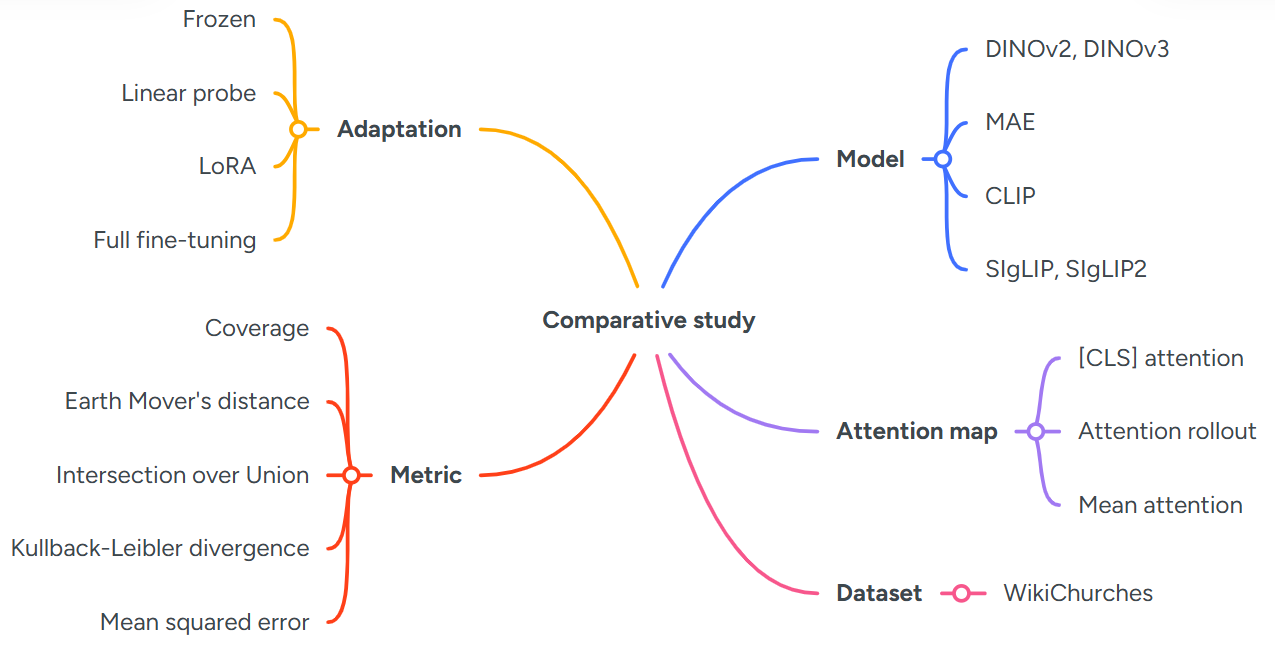
\includegraphics[width=\textwidth]{framework_v1.png}
\caption{A conceptual overview of the experimental pipeline in this study. It compares 6 models, 3 types of attention maps, 4 adaptation strategies, and 5 performance metrics on 1 benchmark dataset. \label{figure framework overview}}
\end{figure}

\subsection{Dataset}

The primary dataset used in this study is WikiChurches~\cite{Barz21WikiChurches}, a fine-grained architectural-style dataset of European church buildings. Its annotation file defines 106 architectural feature types, including arches, windows, towers, and portals, and provides bounding-box annotations with normalized coordinates.

This study uses two data scopes. First, we use an expert-annotated evaluation subset containing 139 images and 631 bounding boxes across four architectural styles: Romanesque~(51 images), Gothic~(49 images), Renaissance~(22 images), and Baroque~(17 images). This subset is used exclusively for attention-alignment evaluation. Second, we use a larger style-labelled pool from the official 9,485-image release for downstream fine-tuning. To prevent data leakage, all 139 expert-annotated images are excluded from the fine-tuning splits.

\textcolor{red}{TJ: Need to add a figure to show image examples. Give me 1 example per style, 4 images in total}

\subsection{Models studied in this paper}

In this paper, we compare six vision foundation models spanning image-only self-supervised models and vision-language models. The image-only models include DINOv2~\cite{Oquab24DINOv2}, DINOv3~\cite{Simeoni26DINOv3}, and MAE~\cite{He22MAE}. The vision-language models include CLIP~\cite{Radford21CLIP}, SigLIP~\cite{Zhai23SigLIP}, and SigLIP2~\cite{Tschannen25SigLIP2}; for these models, we analyze only their visual encoders. DINOv2 uses a patch size of~14, producing a $16\times16$ spatial grid with four register tokens. All other models use a patch size of~16, producing a $14\times14$ spatial grid.

We compare three attention extraction methods, as summarized in Table~\ref{table attention method list}. The first method uses \texttt{[CLS]}-token attention, and the second uses attention rollout. These two methods are applied to DINOv2, DINOv3, MAE, and CLIP, which provide a \texttt{[CLS]}-token pathway. The third method uses a mean-attention proxy and is applied to SigLIP and SigLIP2, which do not provide an equivalent \texttt{[CLS]}-token pathway.


\begin{table}[!h]
\centering \caption{A list of attention extraction methods used in this study. \label{table attention method list}}
\begin{tabular}{ccc}
\toprule
Attention method & Vision foundation model & Remark \\ \midrule
\texttt{[CLS]} attention & DINOv2, DINOv3, MAE, CLIP & Native \texttt{[CLS]} token \\
Rollout & DINOv2, DINOv3, MAE, CLIP & Cross-layer composition \\
Mean attention & SigLIP, SigLIP2 & Proxy (no \texttt{[CLS]} token) \\
\bottomrule
\end{tabular}
\end{table}

We compare three adaptation strategies. First, in the \textit{linear probe setting}, the pretrained backbone is frozen, and only a newly added classification head is trained, providing a lightweight evaluation of the separability of the frozen representations. Second, in the \textit{LoRA setting}, low-rank trainable adapters are inserted into selected layers while the original backbone parameters remain frozen, enabling parameter-efficient adaptation. Third, in the \textit{full fine-tuning setting}, all model parameters are updated on the downstream task, allowing the entire visual representation to be optimized for architectural style recognition.


% \begin{table}[!h]
% \centering
% \caption{A list of adaptation strategies used in this study. \label{table adaptation list}}
% \begin{tabular}{ccc}
% \toprule
% Strategy & Backbone & Role \\ \midrule
% Linear probe & Frozen & Control (zero attention change) \\
% LoRA         & Mostly frozen & Efficient adapter \\
% Full fine-tuning   & Updated end-to-end & Maximum adaptation \\
% \bottomrule
% \end{tabular}
% \end{table}

\subsection{Performance metrics}

\textcolor{red}{TJ: Provide a self-contained formula for these five metrics based on the same notation, such as $A$, $M$, $G$}

Five metrics are used in this study. Let $A$ denote the attention heatmap, $M$ the union binary mask of expert boxes, and $G$ a Gaussian soft-union target derived from the boxes \textcolor{red}{TJ: What Gaussian function is used?}.
\begin{itemize}
    \item IoU thresholds $A$ at the exact top-$k$ pixel count via
\texttt{torch.topk} (top~10\% of pixels) and computes overlap with $M$:
\begin{equation}
  \text{IoU} = \frac{|\hat{A} \cap M|}{|\hat{A} \cup M|}, \quad
  \hat{A} = \text{top-}k\text{-pixels}(A).
\end{equation}
A higher IoU value indicates better performance.
\item Coverage is threshold-free: the fraction of total attention energy
inside $M$,
\begin{equation}
  \text{Coverage} = \frac{\sum_{i \in M} A_i}{\sum_i A_i}.
\end{equation}
A higher Coverage value indicates better performance.
\item \textit{Mean Squared Error} (MSE)
\item \textit{Kullback-Leibler} (KL) divergence
\item \textit{Earth Mover's Distance} (EMD)
\end{itemize}
Each metric catches a different failure mode: IoU@90 asks whether the model's top-attended pixels land inside the expert annotations; Coverage asks what fraction of total attention energy falls inside the annotated regions; MSE, KL, and EMD compare the full heatmap against a Gaussian soft-union target, exposing cases where a model looks reasonable under overlap but still places attention mass in the wrong location.

\textcolor{red}{TJ: Provide descriptions to explain these tests.}
The study uses paired t-tests, Wilcoxon signed-rank tests, bootstrap confidence intervals, Cohen's $d$ for paired differences, and Holm multiple-comparison correction. 

\subsection{\textcolor{red}{Baselines and calibration}}

\textcolor{red}{TJ: I don't understand why we need baseline and calibration}

Continuous metrics are calibrated against four naive baselines: random attention, center Gaussian, saliency prior, and Sobel edge map (Table~\ref{tab:baselines}). Beating random only is weak evidence; clearing all four baselines is stronger support for non-trivial semantic alignment.

\begin{table}[!h]
\centering
\caption{Dataset-level mean baseline scores (lower is better). \textcolor{red}{TJ: Do we need to provide IoU and coverage?}}
\label{tab:baselines}
\begin{tabular}{lccc}
\toprule
Baseline & MSE & KL divergence & EMD \\
\midrule
Random         & 0.3192 & 3.3627 & 0.3468 \\
Center Gaussian & 0.1770 & 2.6317 & 0.2836 \\
Saliency Prior & 0.0957 & 2.6111 & 0.2654 \\
Sobel Edge     & 0.0376 & 3.2237 & 0.3137 \\
\bottomrule
\end{tabular}%
\end{table}


\section{Experimental results} \label{section results}

\subsection{Implementation details}

\textcolor{red}{TJ: Any \textit{preparation} applied to the dataset? preprocessing? For example, XXX images and xxx annotation instances are used. The box is resized to xxx resolution. }

The 139-image annotated evaluation set spans four architectural styles. Average expert boxes per image are 4.5 overall, but vary by style: Gothic and Romanesque images are more densely annotated (4.2--5.9 boxes/image) than Baroque images (1.8 boxes/image), which limits statistical power for that
subset.

\textcolor{red}{TJ: Need to report all details as much as possible. For example, the DINOv2 model weights are obtained from xxx. During the fine-tuning, it is tuned for the downstream dataset xxx. A linear classifier is added on the frozen backbone, and it is tuned using the optimizer AdamW with cosine learning rate scheduling and early stopping on validation accuracy, and trained for xxx epochs. The LoRA adapter is implemented using xxx parameters, attached to the xxx layer. All experiments are implemented using PyTorch XXX version, a server with XXX CPU, XXX GPU. }

All ViT models use ViT-Base scale. Fine-tuning used AdamW with cosine learning rate scheduling, early stopping on validation accuracy. LoRA adapters are inserted into attention projection layers. Heatmaps are computed at a standardised resolution and cached to HDF5/SQLite for fast backend serving. IoU@90 denotes IoU at the top-10\% pixel threshold. Directions: higher is better for IoU and Coverage; lower is better for MSE, KL, and EMD. Results are reported at each model's best default-method layer over the 139 annotated images.

\subsection{Results from RQ1: the behavior of frozen pretrained models}

For RQ1, we evaluate attention alignment in frozen pretrained models before any task-specific adaptation. Five metrics are used to assess alignment from complementary perspectives: IoU and Coverage measure spatial overlap with expert-marked regions, while MSE, KL divergence, and EMD measure distributional similarity between model attention maps and expert annotations. Table~\ref{table RQ1 result} summarizes the results.

Overall, DINOv3 achieves the strongest frozen-model alignment. It obtains the best performance on IoU, Coverage, KL divergence, and EMD, indicating that its attention maps overlap more strongly with expert-marked architectural regions and are also closer to the expert annotations at the distributional level. However, DINOv3 does not achieve the lowest MSE. Instead, SigLIP2 obtains the best MSE score, followed closely by SigLIP. This difference suggests that attention alignment should not be reduced to a single metric: a model may produce locally smooth attention maps with low pixel-wise error while still placing attention mass in less accurate spatial locations.

Among the remaining models, DINOv2 provides the second-best EMD and competitive IoU, suggesting relatively strong spatial localization among the frozen models. MAE performs moderately on IoU and Coverage but has the highest MSE, indicating weaker pixel-level agreement with expert annotations. CLIP shows relatively low IoU and Coverage, suggesting limited spatial overlap between its frozen attention maps and expert-marked regions. SigLIP and SigLIP2 achieve the lowest MSE values, but their higher KL divergence and EMD scores indicate that their attention distributions remain less well aligned with expert annotations despite favorable pixel-wise error.

\begin{table}[!h]
\centering
\caption{Results from RQ1 frozen pretrained models.\label{table RQ1 result}}
\begin{tabular}{cccccc}
\toprule
Vision foundation model & IoU $\uparrow$ & Coverage $\uparrow$ & MSE $\downarrow$ & KL divergence $\downarrow$ & EMD $\downarrow$ \\ \midrule
DINOv2    & 0.082 & 0.100 & 0.021 & 2.684 & 0.298 \\
DINOv3     & 0.133 & 0.137 & 0.027 & 2.325 & 0.260 \\
MAE        & 0.070 & 0.090 & 0.048 & 2.756 & 0.318 \\
CLIP      & 0.049 & 0.085 & 0.021 & 2.912 & 0.326 \\
SigLIP    & 0.074 & 0.076 & 0.018 & 3.002 & 0.348 \\
SigLIP2   & 0.047 & 0.071 & 0.017 & 3.071 & 0.354 \\ \bottomrule
\end{tabular}
\end{table}

Since DINOv3 achieves the strongest overall alignment in Table~\ref{table RQ1 result}, we further examine whether its advantage is consistent with its model design. We hypothesize that DINOv3 benefits from the combination of large-scale self-supervised training and a training recipe intended to preserve dense spatial representations. The DINOv3 technical report~\cite{Simeoni26DINOv3} identifies dense-feature degradation as a potential failure mode during long self-supervised training and introduces Gram anchoring to stabilize patch-level feature maps. Because the RQ1 metrics explicitly reward spatial correspondence between model attention and expert-marked architectural regions, a training strategy designed to preserve dense features provides a plausible explanation for DINOv3's stronger alignment.

To further assess DINOv3's advantage, we conduct two additional checks, summarized in Table~\ref{table RQ1 dinov3}. The first check evaluates robustness. Paired image-level comparisons show that DINOv3 remains consistently ahead of the next-best model across all headline metrics, with Holm-adjusted $p < 1.31 \times 10^{-7}$. This indicates that the observed advantage is not merely a leaderboard artifact caused by aggregation over images. The second check examines where DINOv3 performs best. If DINOv3 preserves cleaner patch-level spatial structure, its attention should align more strongly with mid- to large-scale architectural elements while remaining less effective for small ornamental details. This pattern is consistent with our observations: DINOv3 performs strongest on visually prominent styles such as Gothic and Romanesque, aligns well with large coherent features such as ornate portals and tracery roses, but remains weak on small decorative elements such as crockets, fleurons, and pinnacles.

\begin{table}[!h]
\centering
\caption{Additional robustness and spatial checks for DINOv3. For lower-is-better metrics, the reported gap is computed as the next-best model score minus the DINOv3 score.\label{table RQ1 dinov3}}
\begin{tabular}{lp{0.3\textwidth}p{0.4\textwidth}}
\toprule
Check & Result & Remarks \\ \midrule
Paired gap & $+$0.0425 IoU, $+$0.0330 Coverage, $+$0.3595 KL, $+$0.0378 EMD & It is measured as paired improvement over next-best model. The lead is not an aggregation artifact. \\
Strongest styles & Gothic: 0.169; Romanesque: 0.160 & Alignment is highest for visually prominent structural styles. \\
Strongest features & Ornate Portal: 0.214; Tracery Rose: 0.164 & Attention aligns well with large, coherent architectural parts. \\
Weakest features & Crocket; Fleuron; Pinnacle & Small ornamental details remain challenging. \\
\bottomrule
\end{tabular}
\end{table}


\subsection{Results from RQ2: the internal structure of attention across layers and heads}

RQ2 defines \emph{descriptive specialisation} as a head whose \texttt{[CLS]}-to-patch attention map consistently aligns better than other heads with expert-marked regions or feature labels. It is not a causal-attribution claim. The scope is the architecture-native \texttt{[CLS]}-token ViTs: DINOv2, DINOv3, MAE, and CLIP; SigLIP, SigLIP2, and ResNet-50 are excluded because their per-head proxies do not use native attention heads, and rollout is excluded because it aggregates layers. Heads are ranked primarily by IoU@90, with Coverage and EMD as robustness checks.

\subsubsection{A study on various layers}

A study on various layers is provided in Table \ref{figure RQ2 layer ranking}.

\begin{figure}[!h]
\centering
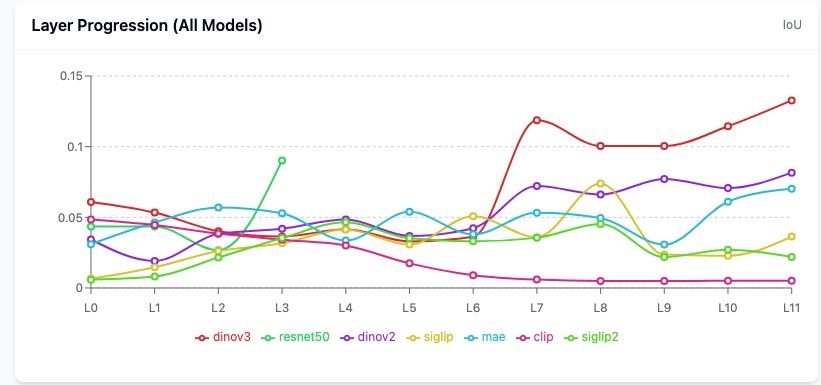
\includegraphics[width=\linewidth]{RQ2_layer_iou.png}
\caption{Layer ranking. \textcolor{red}{TJ: I cropped this image. Please give me a new image, enlarge the text font, remove resnet, change the order of six models to be consistent.}}
\label{figure RQ2 layer ranking}
\end{figure}


\subsubsection{A study on various heads}

Head Ranking identifies a dominant head shown in Figure \ref{figure RQ2 feature matrix}; the Head-Feature Matrix asks what architectural evidence that head aligns with. The observation is that the strongest heads mostly align with larger, coherent structural features. For DINOv3, the same \texttt{layer10/head8} that leads the ranking view also carries the selected \emph{Columned Portal} cell at IoU@90~$=$~0.215 across 15 annotations, linking the ranking evidence to the feature evidence.

\begin{figure}[!h]
\centering
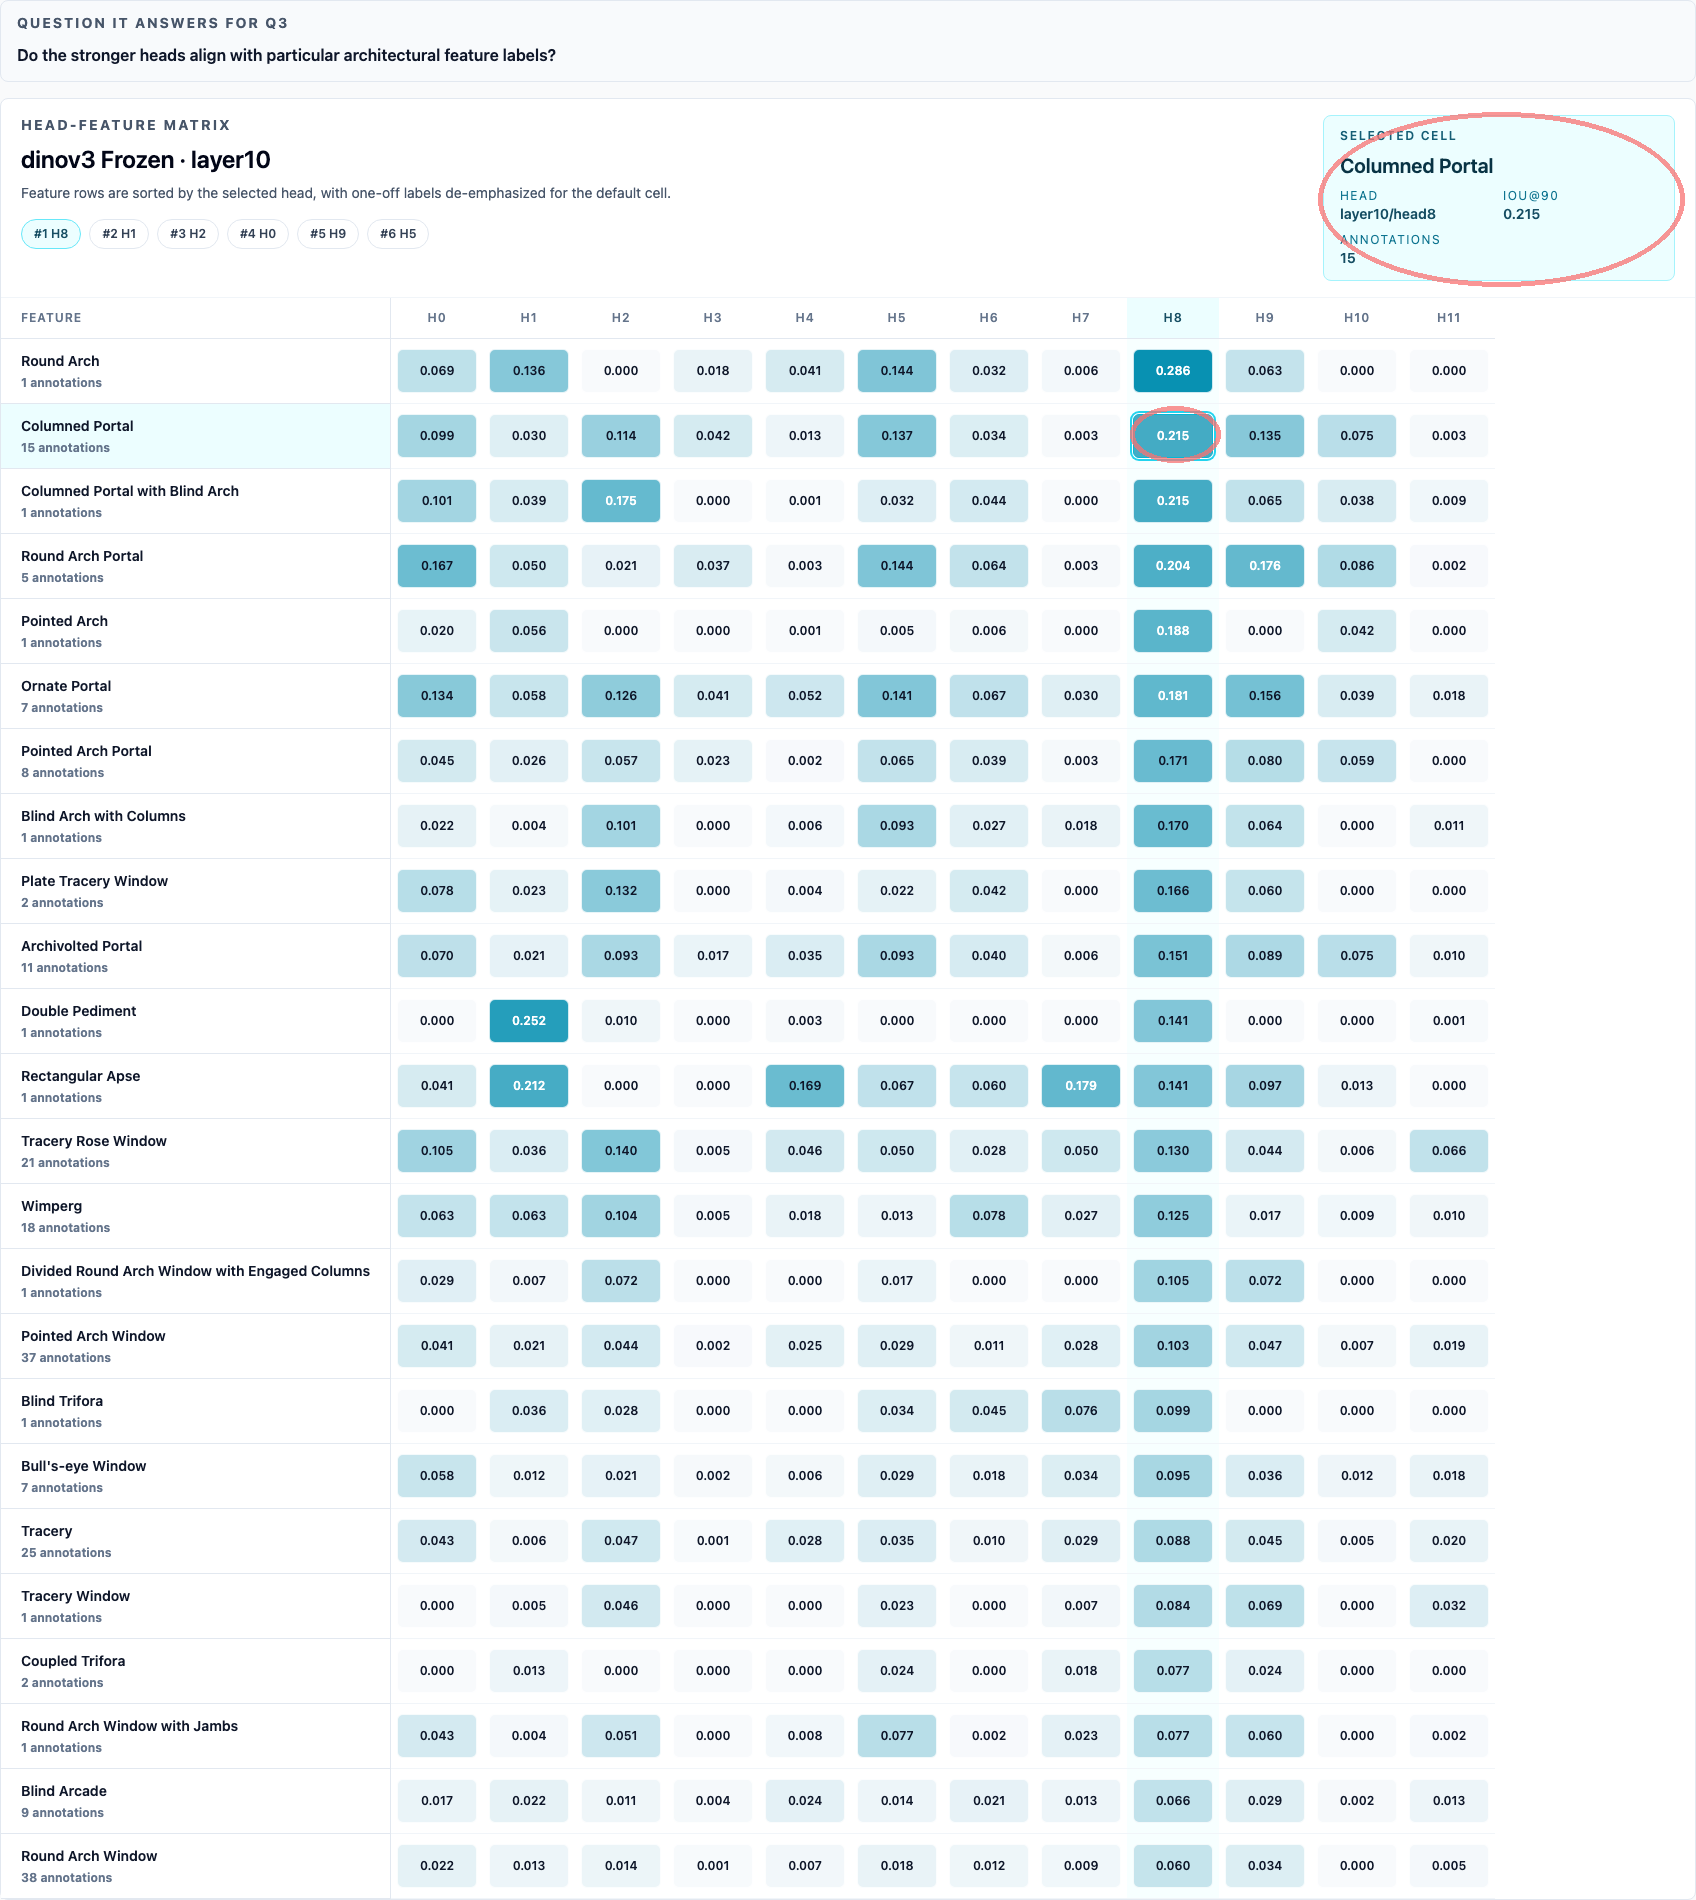
\includegraphics[width=\textwidth]{RQ2_head_feature_matrix_report_view.png}
\caption{RQ2. Head-Feature Matrix report view for DINOv3 frozen attention (\texttt{layer = 10}, IoU@90). The same \texttt{head8} that leads the ranking view also carries the selected \emph{Columned Portal} cell at IoU@90~$=$~0.215 across 15 annotations: the dominant head is strongest on portal-scale structure. \textcolor{red}{TJ: Remove the red circle. Explain the meaning of colors. Possible to increase text font size?}}
\label{figure RQ2 feature matrix}
\end{figure}

To keep the visual check disciplined, for each scoped model, we take its frozen IoU@90 dominant head from the ranking view and sort architectural features for that head with at least three annotations. Figure~\ref{figure RQ2 top bottom} shows the three strongest and three weakest
features for each model's dominant head.

\begin{figure}[!h]
\centering
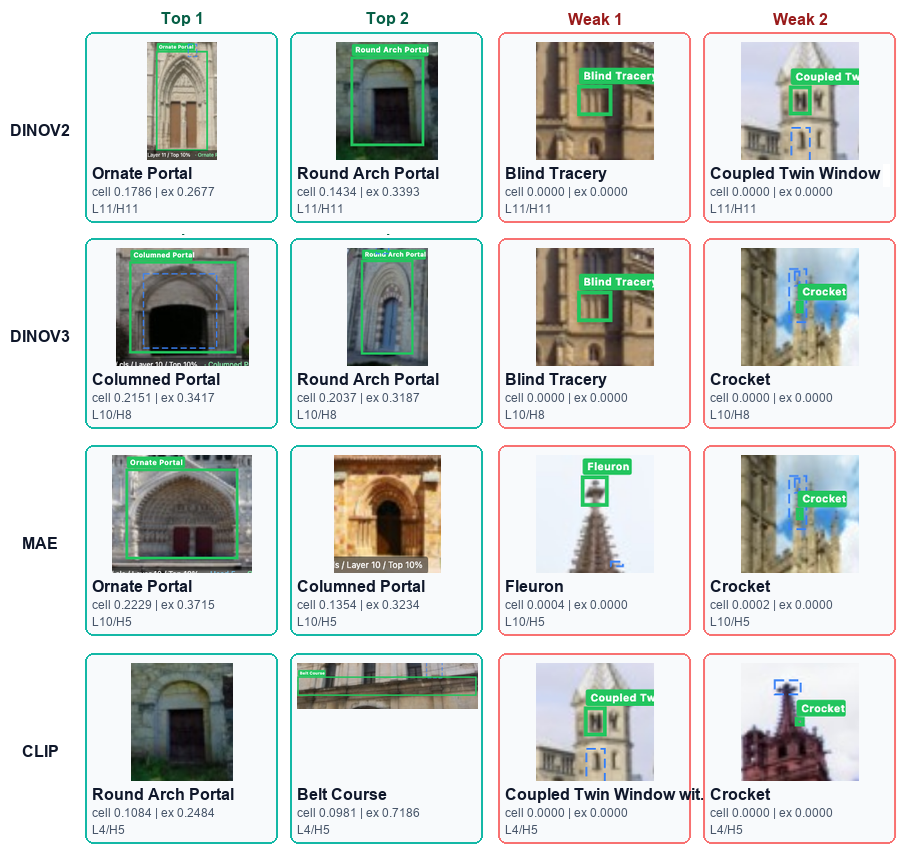
\includegraphics[width=\textwidth]{RQ2_head_feature_top_bottom_4_examples.png}
\caption{The frozen dominant IoU@90 head in each scoped model: DINOv3 \texttt{layer10/head8}, DINOv2 \texttt{layer11/head11}, MAE \texttt{layer10/head5}, CLIP \texttt{layer4/head5}. Strongest features are dominated by portal-scale or facade-structure parts (\emph{Columned Portal}, \emph{Round Arch Portal}, \emph{Ornate Portal}, \emph{Wimperg}, \emph{Belt Course}). Weakest features are thin or decorative labels (\emph{Blind Tracery}, \emph{Crocket}, \emph{Tabernacle}, \emph{Fleuron}, \emph{Coupled Twin Window with Discharging Arch}, \emph{Projecting Cornice}). \textcolor{red}{TJ: I edited this photo to show 4 examples only. Shall we add SIgLIP, SIgLIP2?}}
\label{figure RQ2 top bottom}
\end{figure}

Across the four scoped models, the pattern is consistent. DINOv3's \texttt{layer10/head8} reaches mean feature-level IoU@90 of 0.215 on \emph{Columned Portal}, 0.204 on \emph{Round Arch Portal}, and 0.181 on \emph{Ornate Portal}, while its weakest supported features are essentially zero on \emph{Blind Tracery}, \emph{Crocket}, and \emph{Tabernacle}. DINOv2 shows the same portal-heavy top end and the same small-detail failure boundary. MAE also favours large facade parts, but its third-strongest feature is \emph{Wimperg}, fitting the RQ2 observation that MAE is more responsive to compact geometric forms. CLIP's inclusion of \emph{Belt Course} suggests feature extent and clean geometry matter, not only semantic category names.

The strongest heads are therefore better described as heads whose spatial patterns are more compatible with expert-marked \emph{structural} parts rather than as exact part detectors, and the failure cases are not random: across families, the weak features tend to be small, thin, repeated, or visually entangled with surrounding masonry.

\subsection{Results from RQ3: The effect of downstream adaptation}

Linear Probe produces exactly zero $\Delta$ across all metrics for all models, confirming that observed RQ3 movement is tied to actual representation change rather than a reporting artefact. Figure~\ref{figure RQ3 heatmap} shows the multi-metric improvement heatmap across all non-Linear-Probe combinations. Figure~\ref{figure RQ3 forest} adds the statistical layer with bootstrap confidence intervals.

\begin{figure}[!h]
\centering
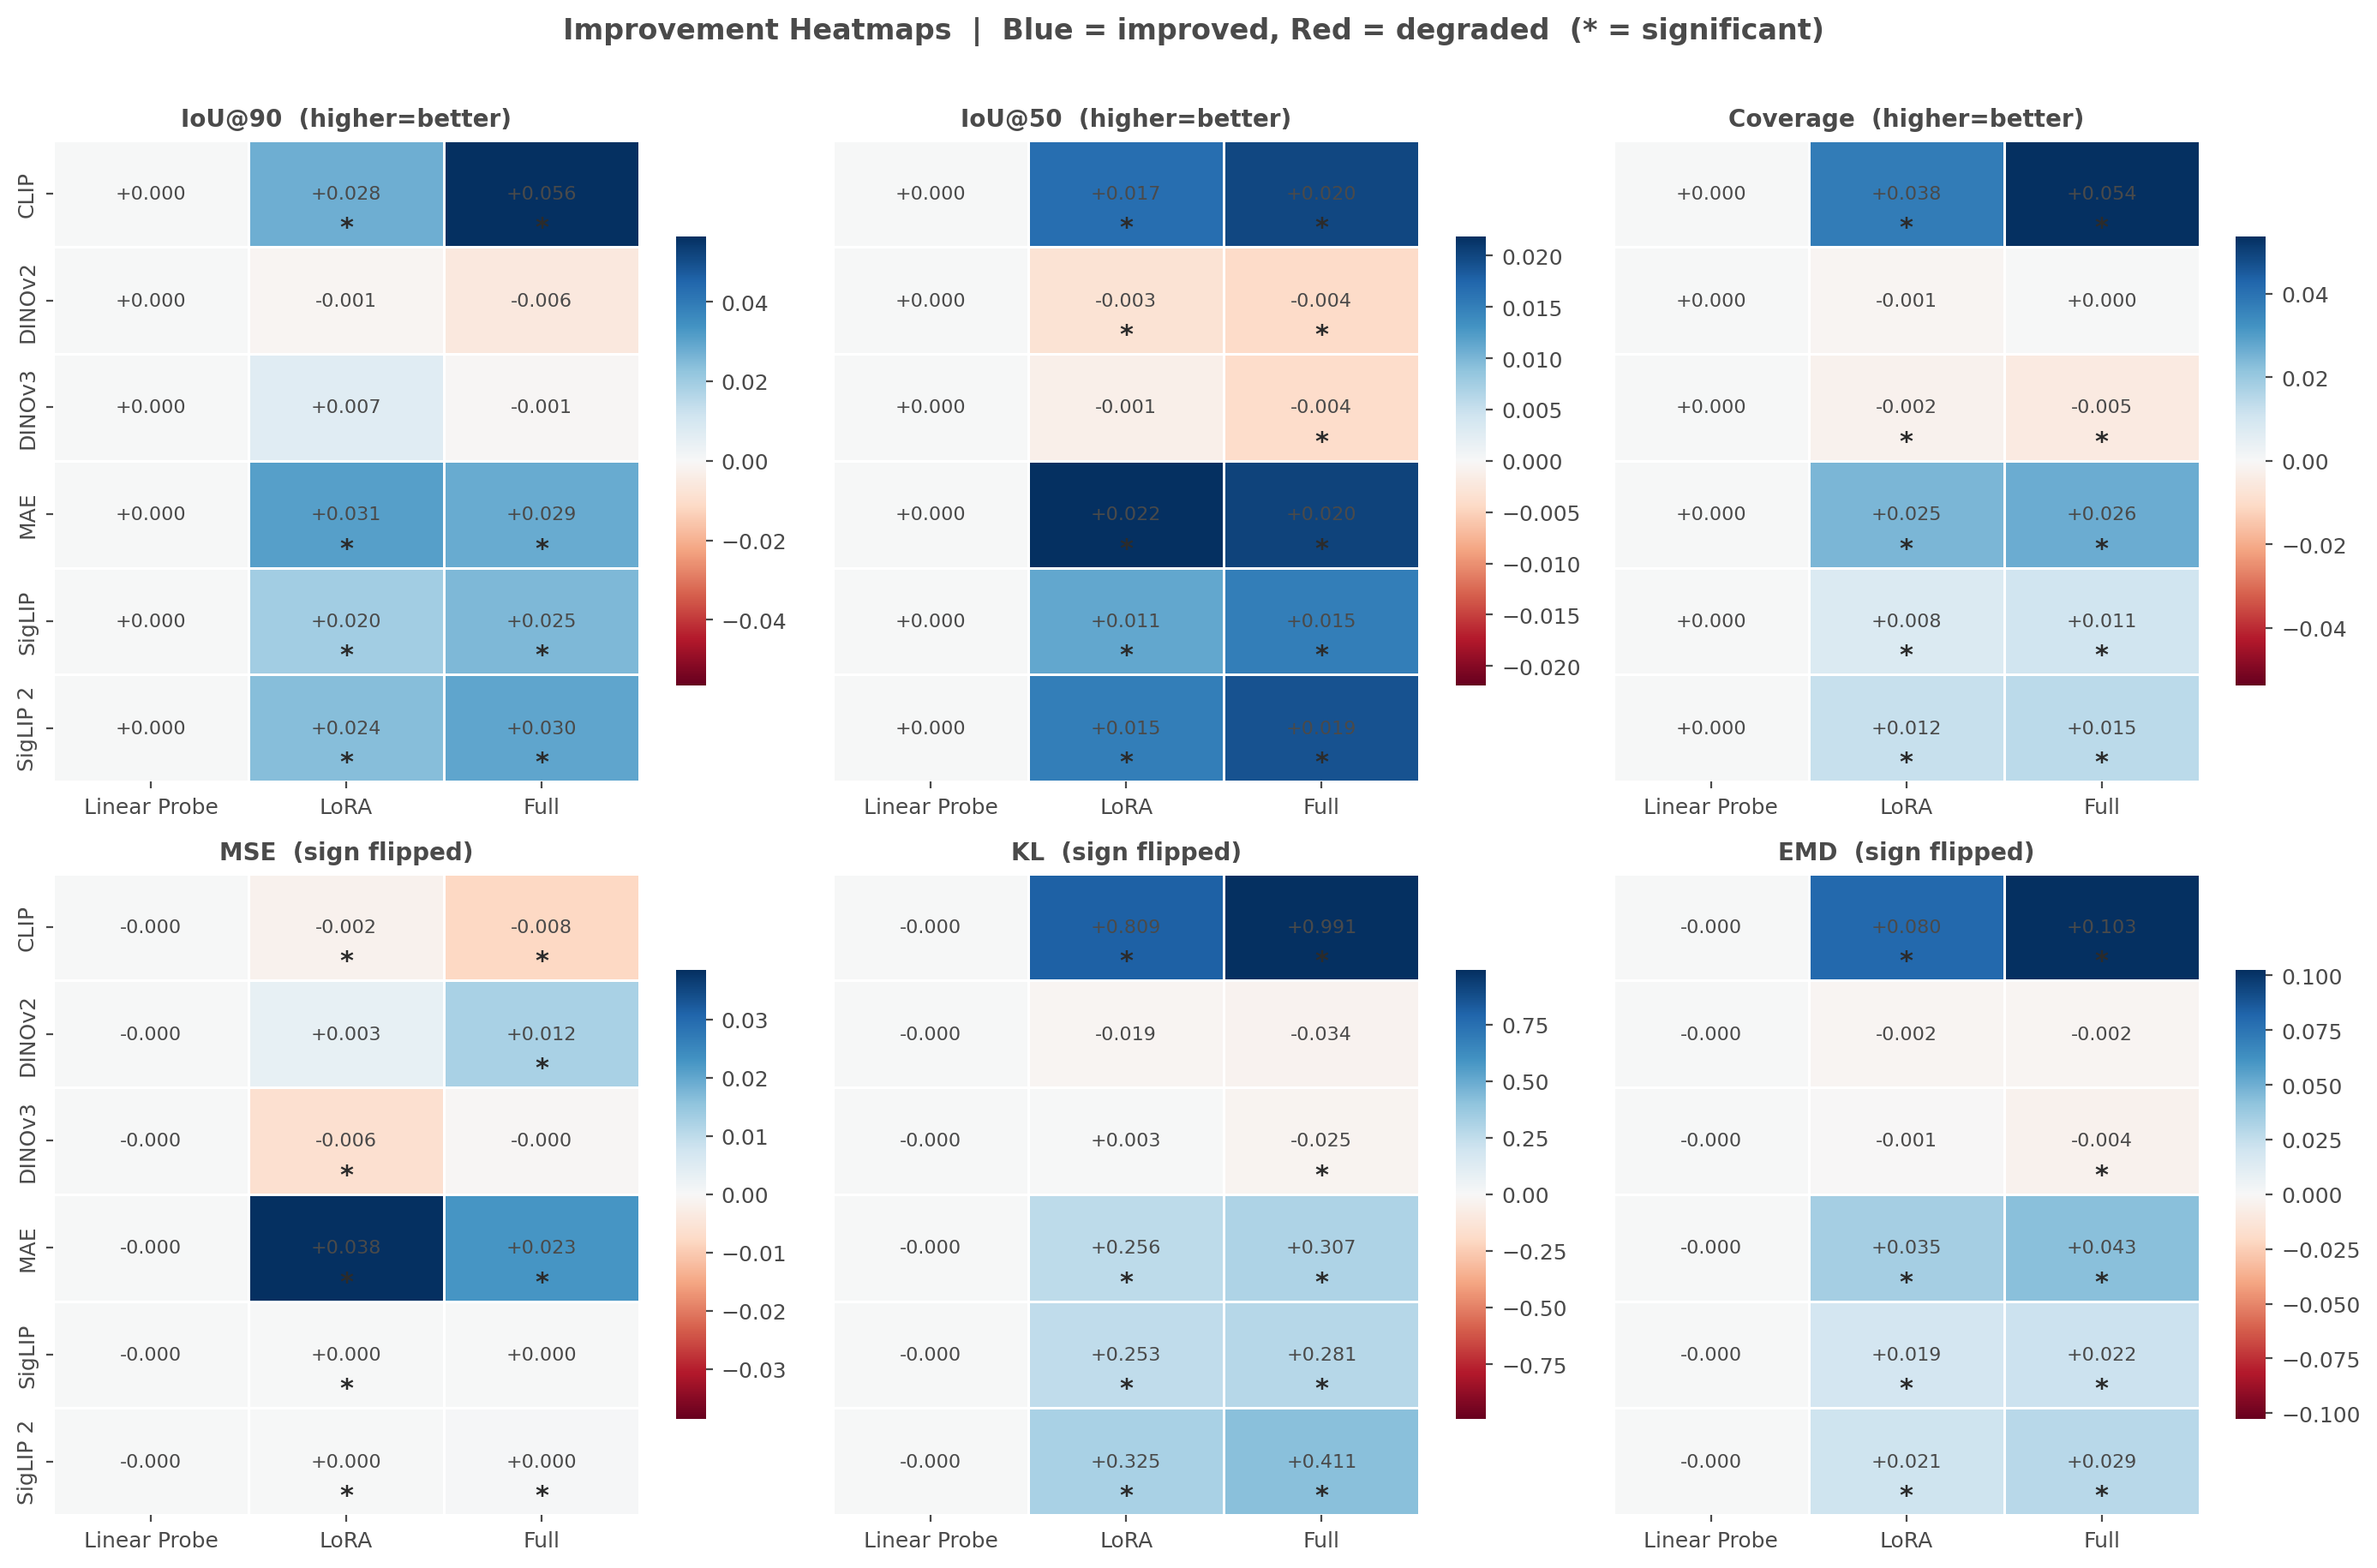
\includegraphics[width=\textwidth]{RQ3_all_metrics_improvement_heatmap.png}
\caption{multi-metric improvement heatmap. Each cell shows whether LoRA or Full fine-tuning enhances, preserves, or degrades alignment relative to the frozen model. \textcolor{red}{TJ: all results use the same order, DINOv2, DINOv3, MAE, CLIP, SIgLIP, SIgLIP2. Enlarge text fonts. Enlarge the height of the right legend bar}}
\label{figure RQ3 heatmap}
\end{figure}


\begin{figure}[!h]
\centering
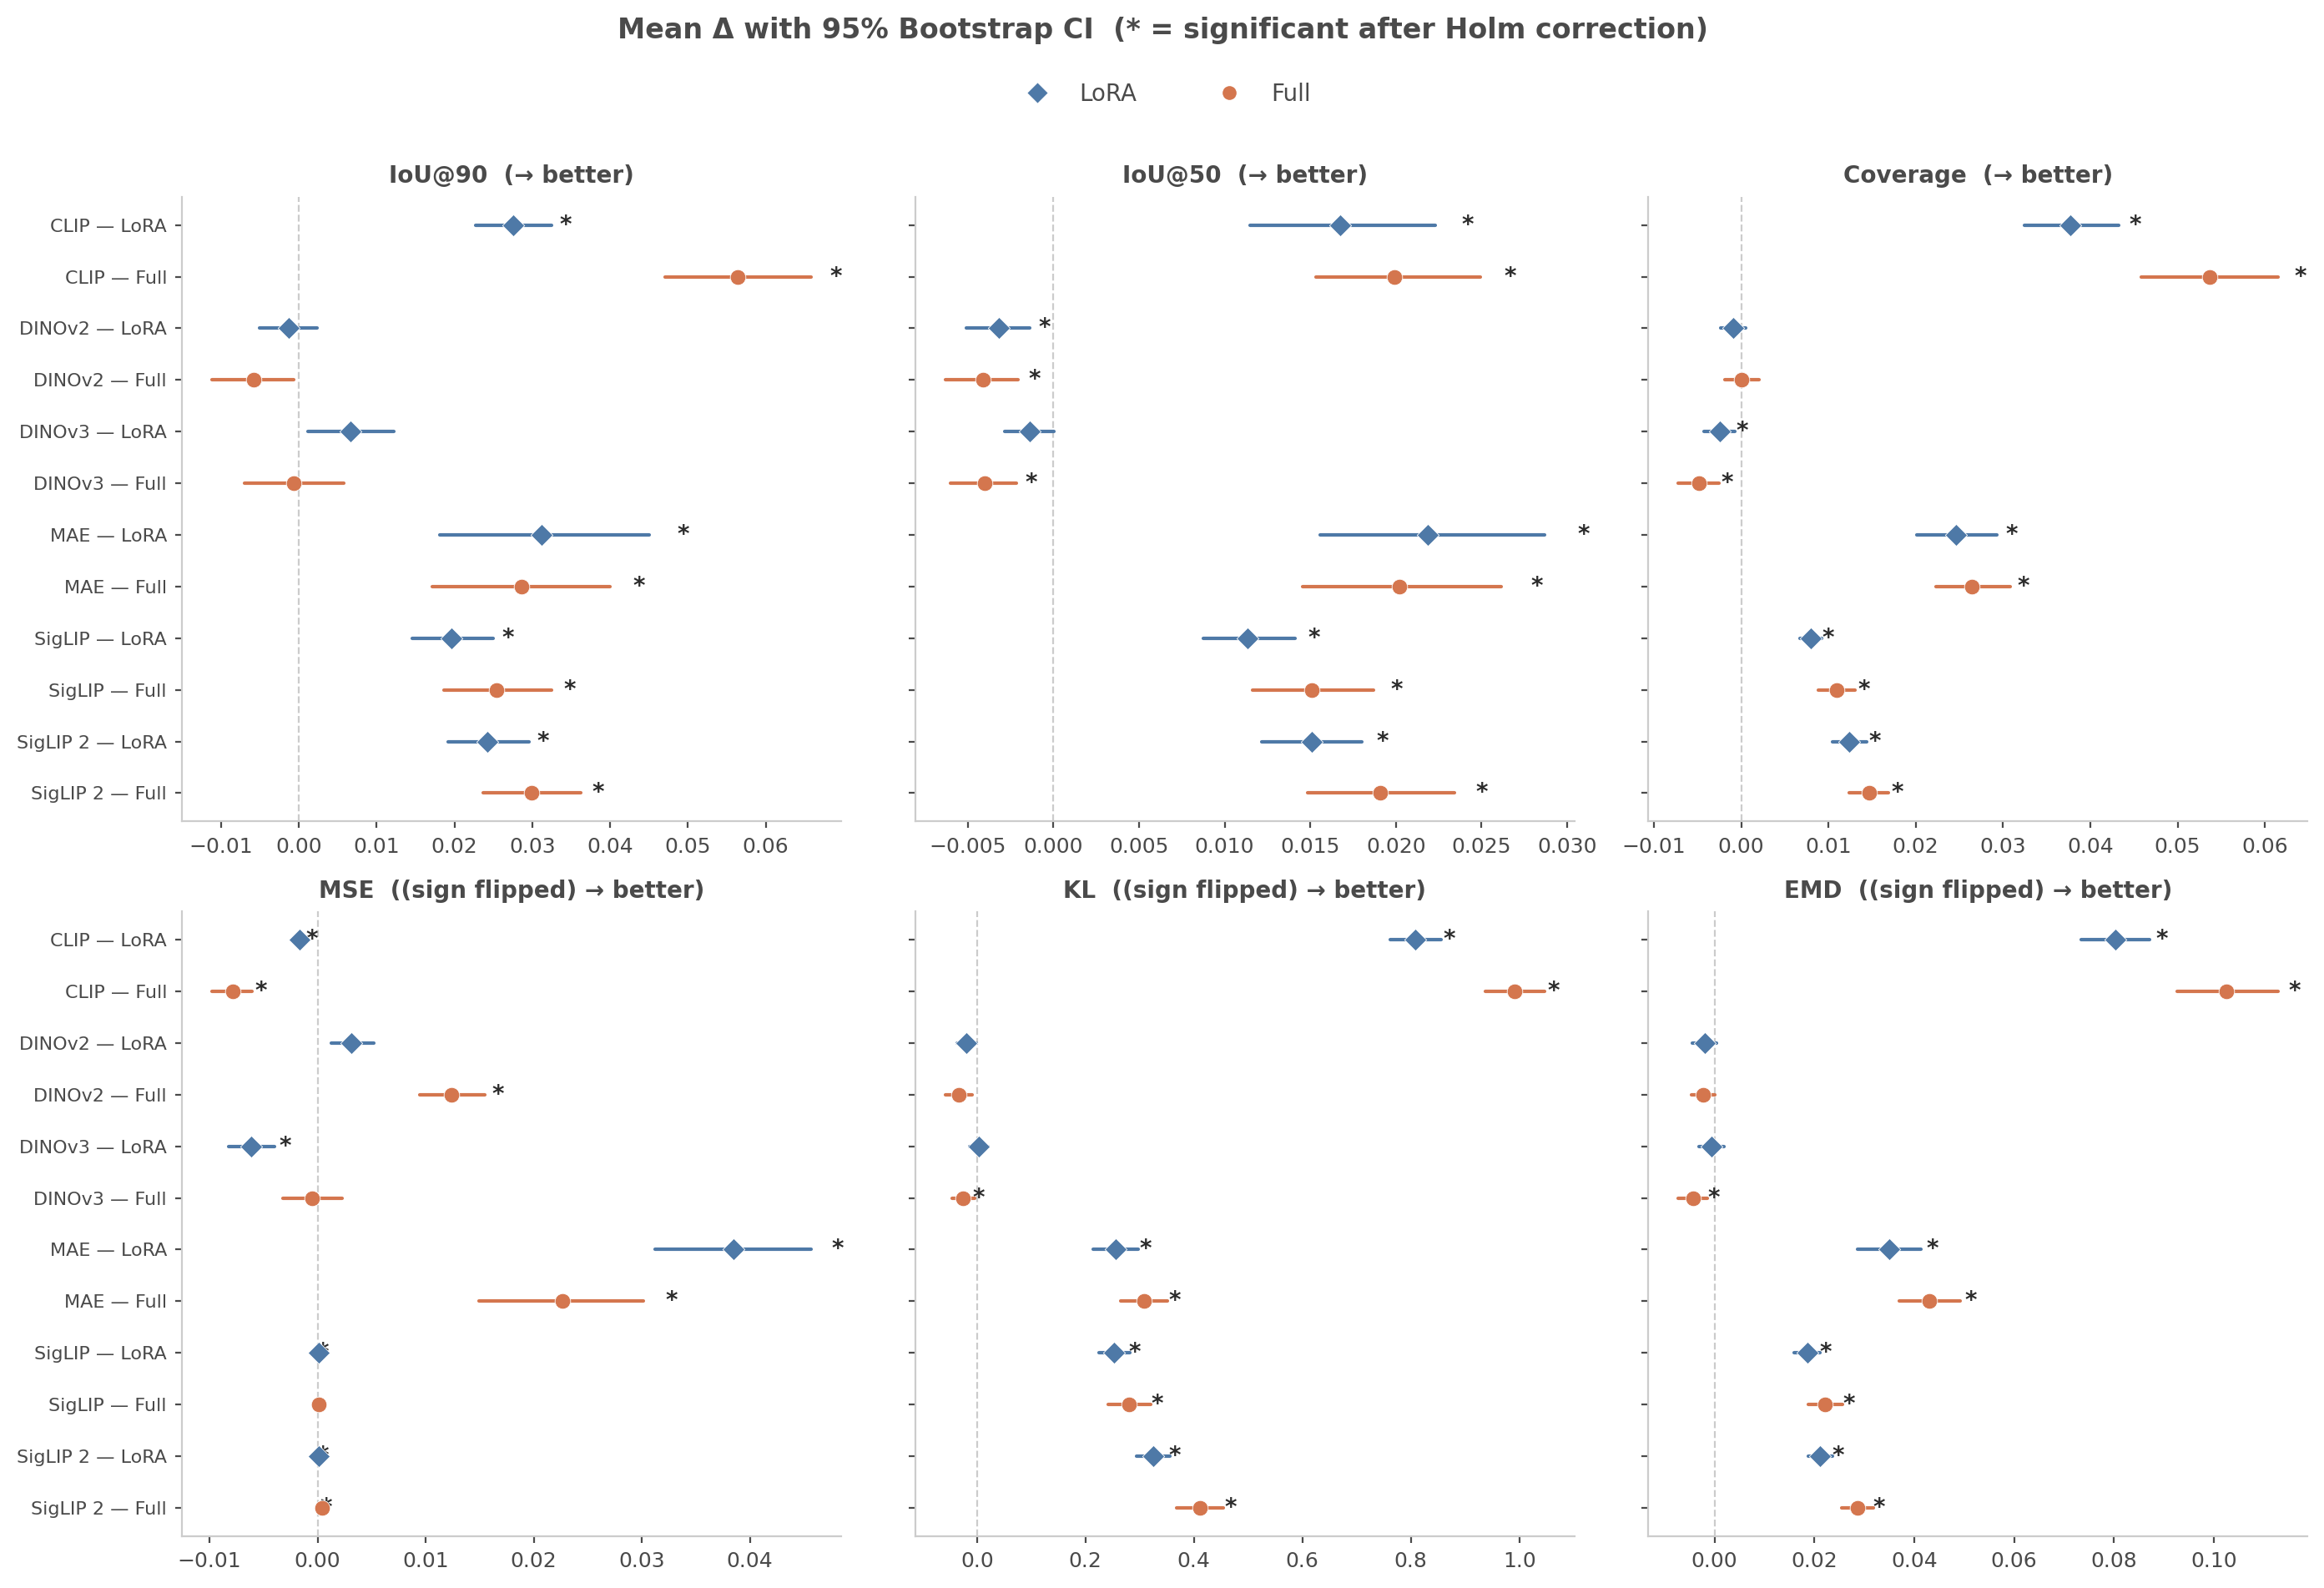
\includegraphics[width=\textwidth]{RQ3_forest_plot_ci.png}
\caption{Forest plot of $\Delta$IoU@90 with 95\% bootstrap confidence intervals per model and strategy. \textcolor{red}{TJ: Is it a detail for Figure \ref{figure RQ3 heatmap}? Adjust the y-axis to use the same order, DINOv2, DINOv3, MAE, CLIP, SIgLIP, SIgLIP2.}}
\label{figure RQ3 forest}
\end{figure}

\begin{table}[!h]
\centering
\caption{Per-style $\Delta$IoU@90 under Full fine-tuning.}
\label{table RQ3 perstyle}
\begin{tabular}{lcccc}
\toprule
Vision foundation model & Romanesque & Gothic & Renaissance & Baroque \\ \midrule
DINOv2  & $-$0.010 & +0.001 & $-$0.004 & $-$0.012 \\
DINOv3  & $-$0.001 & +0.006 & $-$0.004 & $-$0.009 \\
MAE     & +0.007 & +0.009 & +0.108 & +0.045 \\
CLIP    & +0.066 & +0.079 & +0.014 & +0.013 \\
SigLIP  & +0.029 & +0.039 & $-$0.006 & +0.005 \\
SigLIP2 & +0.034 & +0.044 & +0.007 & +0.007 \\
\bottomrule
\end{tabular}
\end{table}


CLIP shows the largest gain (Full fine-tuning: IoU $0.0181\!\to\!0.0745$, Coverage $0.051\!\to\!0.105$, Cohen's $d\!\approx\!1.0$). The per-style breakdown (Table~\ref{table RQ3 perstyle}) reveals that virtually all of CLIP's gain concentrates on Romanesque (+0.066) and Gothic (+0.079) images, whose diagnostic features (Round Arch Portals, Pointed Arch Portals, Tracery) appear frequently in English-language web text - consistent with CLIP's language-grounded training. Renaissance (+0.014) and Baroque (+0.013) show near-zero gain.

A Kruskal-Wallis test finds significant style moderation for CLIP ($p\!=\!7.2\!\times\!10^{-9}$), MAE ($p\!=\!3.8\!\times\!10^{-7}$), SigLIP ($p\!=\!1.5\!\times\!10^{-5}$), and SigLIP2 ($p\!=\!5.0\!\times\!10^{-7}$); DINOv2 and DINOv3 are not significant ($p\!=\!0.18$, $p\!=\!0.12$), consistent with their near-zero per-style profiles.

\textbf{MAE}'s Renaissance $\Delta$ of +0.108 is the largest single-style shift in the dataset. The two most common Renaissance features (Pilaster, Belt Course) show negative $\Delta$, suggesting the style-classification gradient routes attention toward the most discriminative geometric forms.

\textbf{SigLIP variants.} \textcolor{red}{TJ: which figure/table is used to get this analysis?} The RQ2 analysed layer is \texttt{layer11}, where both SigLIP and SigLIP2 start from weaker frozen IoU@90 baselines than the DINO family (\texttt{siglip} 0.0364, \texttt{siglip2} 0.0220). Under Full fine-tuning, base SigLIP remains higher in absolute IoU@90 (0.0618 vs.\ SigLIP2 0.0519), but SigLIP2
moves further in standardised-effect terms ($\Delta\!=\!0.0299$, Cohen's $d\!=\!0.781$, vs.\ SigLIP's $\Delta\!=\!0.0254$, $d\!=\!0.604$), consistent with more late-layer adaptation headroom from a weaker starting point and the denser grounding components of SigLIP2.

\textbf{DINO family.} Both DINOv2 and DINOv3 show near-zero $\Delta$ across all styles and strategies. $\Delta\!\approx\!0$ is a positive generalisation result: expert-aligned spatial structure is already encoded by pretraining, and the style-classification gradient is absorbed by the classification head rather than reshaping backbone attention.


\textbf{Cross-model correlation.} DINOv3 frozen IoU predicts CLIP $\Delta$IoU at Pearson $r\!=\!+0.677$ ($\rho\!=\!+0.681$, $p\!<\!0.0001$; see Figure~\ref{figure RQ3 model scatter}): the images CLIP gains on are the same structurally easy images DINOv3 already attends to. Within-cluster language model correlations (CLIP--SigLIP--SigLIP2) are $r\!\approx\!0.43$--$0.58$; MAE is anti-correlated with the language cluster ($r\!\approx\!{-}0.22$ to ${-}0.31$). Models with different pretraining objectives converge on the same structurally easy images rather than specialising on complementary subsets.

\begin{figure}[!t]
\centering
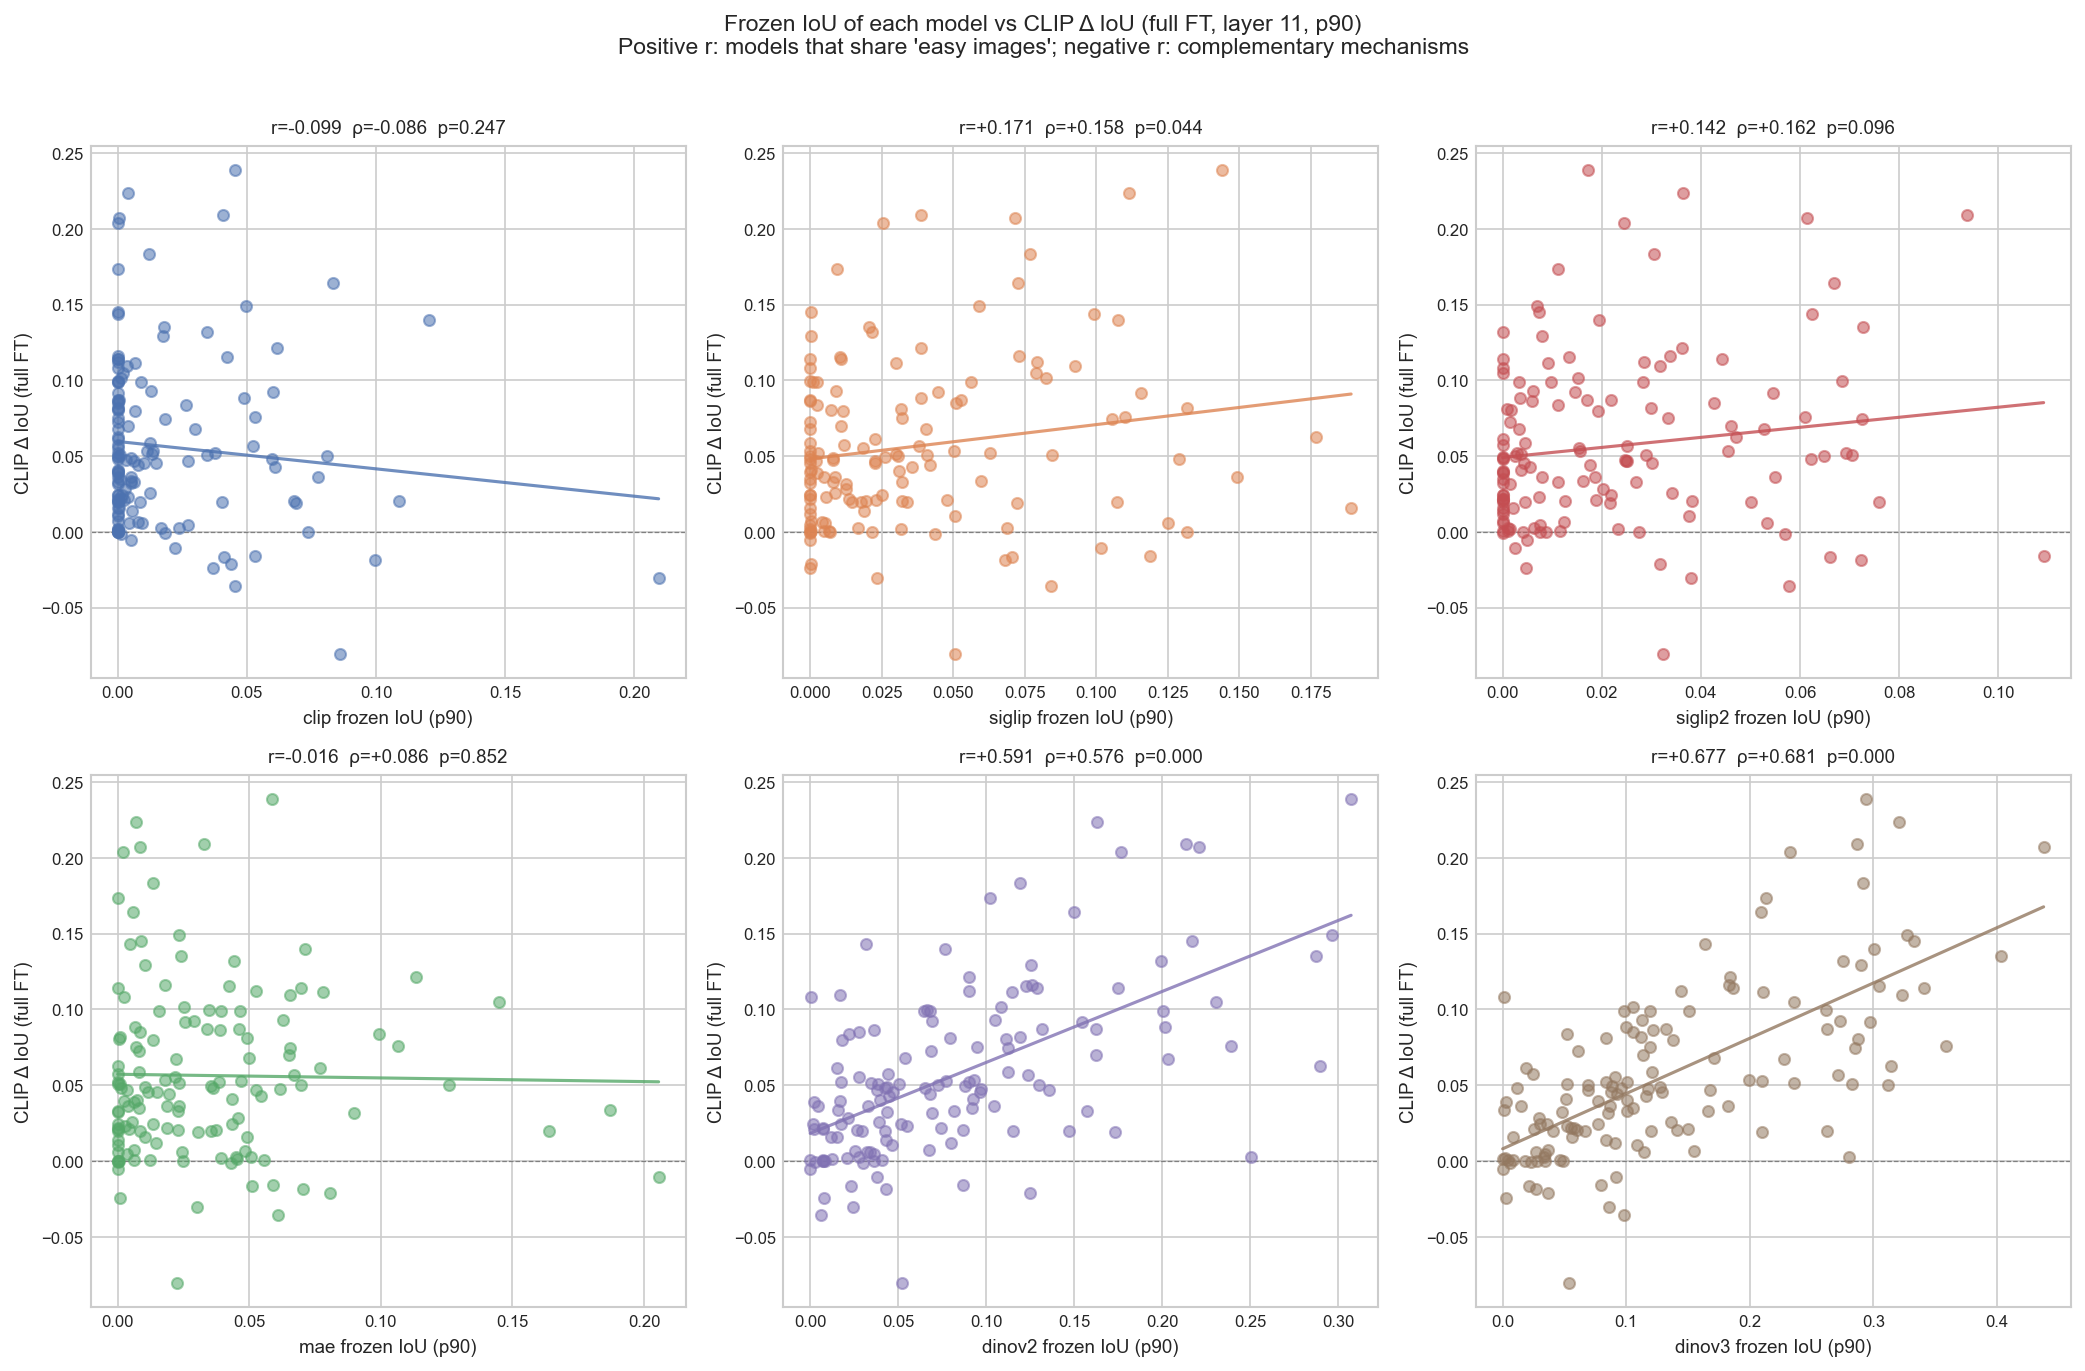
\includegraphics[width=\textwidth]{RQ3_model_correlation_scatter.png}
\caption{DINOv3 frozen IoU@90 vs.\ CLIP $\Delta$IoU@90 per image ($r\!=\!+0.677$). Structural image difficulty, not model family, determines what is ``easy''. \textcolor{red}{TJ: INcrease text font size, remove title}}
\label{figure RQ3 model scatter}
\end{figure}

Expert-aligned attention concentrates in a small number of heads rather than spreading uniformly across the transformer (Figure~\ref{figure RQ3 head ranking}). DINOv3 is the cleanest case: the same \texttt{layer10/head8} remains best across Frozen, LoRA, and Full, appearing in the top three on more than 110 of 139 images in every condition. DINOv2 shows the same preserved-head pattern at lower absolute alignment. MAE shifts from \texttt{layer10/head5} to \texttt{layer11/head7} under LoRA, then returns to \texttt{layer10/head5} under Full. CLIP is the clearest reorganisation case: frozen CLIP's best heads sit in early layers (\texttt{layer4/head5} leads at mean IoU@90~$=$~0.067), while the selected late layer used in the delta view is weak before adaptation (\texttt{layer11} max IoU@90~$=$~0.034) and then becomes the strongest adapted layer (best \texttt{layer11} head reaches 0.084 under LoRA and 0.105 under Full), with \texttt{layer4/head5} staying near its frozen score. Coverage and EMD agree on the high-level reading, with DINO-family stability being cross-metric while MAE and CLIP preserve only the broader adaptation pattern rather than the exact winning head.



\begin{table}[!h]
\caption{Q3 head-ranking transition map. Each node is the best IoU@90 head for a model variant, with mean IoU@90 and top-3 frequency across the 139 annotated images. DINO-family models preserve their dominant heads across adaptation; MAE shows a mixed pattern; CLIP shifts from an early frozen head to late-layer adapted heads. \textcolor{red}{TJ: I changed your previous figure to be a table. Shall we add SIgLIP, SIgLIP2 and linear probe?}\label{table RQ3 head ranking}}
\begin{tabular}{l|cccccc}
\hline
Vision & \multicolumn{6}{c}{Fine-tuning strategy}  \\
foundation & \multicolumn{2}{c}{Frozen} & \multicolumn{2}{c}{LoRA} & \multicolumn{2}{l}{Full fine-tuning} \\
model & Layer & Head & Layer & Head & Layer & Head \\ \hline
DINOv2 & 10 & 8 & 10 & 8 & 10 & 8 \\
DINOv3 & 11 & 11 & 11 & 11 & 11 & 11 \\
MAE & 4 & 5 & 11 & 11 & 11 & 3 \\
CLIP & 10 & 5 & 11 & 7 & 10 & 5 \\\hline
\end{tabular}
\end{table}

The same concentration pattern holds across the full $12 \times 12$ grid of (layer, head) pairs. In each frozen scoped model, the top-ranked pair's mean IoU@90 lands $2.7\times$--$3.5\times$ above the median pair's (DINOv3 $3.45\times$, CLIP $3.22\times$, MAE $2.92\times$, DINOv2 $2.69\times$). The five best pairs together account for $7.3\%$--$9.0\%$ of total mean IoU@90 across all 144 pairs, roughly $2\times$ the $3.5\%$ they would hold if alignment were uniform. This is the quantitative content of ``sparse'': expert-aligned signal concentrates in a small minority of heads rather than spreading evenly. This connects to Q2. DINO-family models already have strong frozen spatial alignment, so fine-tuning mostly preserves the dominant expert-aligned head. CLIP and MAE gain more from adaptation, and RQ3 shows that those gains can come from \emph{different heads} becoming best aligned after fine-tuning. CLIP's \texttt{layer11} alignment is newly strengthened by adaptation rather than inherited from an already strong frozen \texttt{layer11} head, while MAE is selectively reshaped toward discriminative geometric forms.


\subsection{Summary of key findings}

For \textbf{Q1}, frozen expert-aligned attention exists but is not evenly distributed. DINOv3 provides the strongest evidence, leading the default-method benchmark on IoU, Coverage, KL, and EMD and clearing all calibrated baselines. Base SigLIP is a stronger frozen overlap result than SigLIP2 at its best mean-attention layer, but both variants still have late-layer adaptation headroom. The safest interpretation is not that all SSL models attend like experts, but that DINOv3's spatial prior is unusually compatible with expert-marked architectural evidence in WikiChurches.

For \textbf{Q2}, per-head specialisation is sparse, descriptive, and family-shaped. DINOv3's \texttt{layer10/head8} and DINOv2's \texttt{layer11/head11} remain dominant across Frozen, LoRA, and Full, consistent with the DINO family's already-strong spatial prior. MAE is partly reshaped by adaptation, while CLIP shows the clearest reorganisation from an earlier frozen head to later adapted heads. The strongest head-linked architectural features cluster on portals, arches, and rose-window-scale structures, so the safest claim is not that heads are exact architectural-part detectors, but that some heads expose spatial patterns more compatible with expert-marked structure than others.

For \textbf{Q3}, fine-tuning's effect is mediated by three interacting factors: the pretraining objective's spatial prior (DINO preserves strong frozen alignment; CLIP, MAE, and SigLIP-family gain because they lack it); dataset linguistic coverage (CLIP's gain concentrates on Gothic and Romanesque features densely described in English web text); and geometric discriminability (MAE redirects attention to Renaissance-exclusive pediment forms that pixel reconstruction already encodes with high local fidelity). Models with different objectives converge on the same structurally easy images rather than complementary subsets, with implications for ensembling strategies.

\textbf{Intuitive findings.} Linear Probe as a true attention-change control validates that RQ2 movement reflects representation change, not a reporting artefact. Stronger task-conditioned adaptation helps most when the frozen model is not yet strongly aligned - CLIP, MAE, and SigLIP-family results fit this pattern.

\textbf{Surprising findings.} The SigLIP family pairs excellent frozen MSE with EMD worse than random, illustrating why single-metric interpretation is dangerous. DINOv2 does not improve dramatically under RQ2 despite other families gaining substantially: self-distillation may already produce more part-like spatial attention, leaving less headroom for downstream adaptation.

\textbf{Pretraining objective account.} CLIP's InfoNCE loss~\cite{Radford21CLIP} applies no patch-level spatial pressure; fine-tuning is the first spatial signal, and the gain concentrates on styles whose features are linguistically described. MAE's 75\%-masking objective~\cite{He22MAE} forces precise local geometry representations, which explains its Renaissance pediment affinity. DINOv3's Gram-anchoring loss~\cite{Simeoni26DINOv3} explicitly preserves second-order spatial structure, explaining its $\Delta\!\approx\!0$ result under Q2.


\subsection{Limitations}

The annotated evaluation subset is small (139 images), limiting statistical power. Bounding boxes are expert-guided but not exhaustive, introducing sparse annotation bias, especially for Baroque. Attention is an incomplete explanation signal: strong alignment is evidence of plausibility, not causal proof. IoU depends on the thresholding rule; continuous metrics require calibration to avoid overreading raw numbers.

\section{Conclusions} \label{section conclusions}

This paper asks whether self-supervised vision foundation models attend to the same architectural evidence that experts consider diagnostically important. Using WikiChurches, expert bounding boxes, and a multi-metric alignment framework, we address three linked questions across seven models and three fine-tuning strategies.




%\cite{*}

\backmatter


\section*{Declarations}

\textbf{Funding}

This research received no external funding. \newline

\noindent\textbf{Competing interests}

The authors declare no financial or commercial conflicts of interest. \newline

\noindent\textbf{Ethics approval and consent to participate}

Not applicable.\newline

\noindent\textbf{Consent for publication}

Not applicable.\newline

\noindent\textbf{Data availability }

The dataset that supports the findings of this study is provided in \cite{Barz21WikiChurches}. The data that supports the findings of this study is available on the GitHub repository \url{https://github.com/XXX}.\newline

\noindent\textbf{Code availability }

The code that supports the findings of this study is available on the GitHub repository \url{https://github.com/XXX}.\newline

\noindent\textbf{Author contribution}

% Please choose from the following list. It is okay for multiple authors to choose the same items. No need to cover the entire list because some items are not applicable.

First author: Second author:

J. Tian: Formal analysis, Writing - Original Draft, Writing - Review \& Editing, Supervision.

X. Xie: Formal analysis, Writing - Original Draft, Writing - Review \& Editing.

% Choose from the following list, 
% % https://www.elsevier.com/researcher/author/policies-and-guidelines/credit-author-statement
% Conceptualization
% Methodology
% Software
% Validation
% Formal analysis
% Investigation
% Resources
% Data Curation
% Writing - Original Draft
% Writing - Review \& Editing
% Visualization
% Supervision
% Project administration
% Funding acquisition

%%===========================================================================================%%
%% If you are submitting to one of the Nature Portfolio journals, using the eJP submission   %%
%% system, please include the references within the manuscript file itself. You may do this  %%
%% by copying the reference list from your .bbl file, paste it into the main manuscript .tex %%
%% file, and delete the associated \verb+\bibliography+ commands.                            %%
%%===========================================================================================%%

\bibliography{xvision}% common bib file


\end{document}
